%============================================================================
% BLOC: A Social-First Unified Payments Platform for the Kenyan Market
% Comprehensive Final Year Project Report
% United States International University - Africa
%============================================================================

\documentclass[12pt, a4paper, twoside, openright]{report}

% ============================================================================
% PACKAGES
% ============================================================================

\usepackage[utf8]{inputenc}
\usepackage[T1]{fontenc}
\usepackage[english]{babel}
\usepackage{lmodern}

% Page layout and margins
\usepackage[top=1in, bottom=1in, left=1.25in, right=1.25in]{geometry}
\usepackage{setspace}
\onehalfspacing

% Typography and formatting
\usepackage{graphicx}
\usepackage{subcaption}
\usepackage{float}
\usepackage{booktabs}
\usepackage{array}
\usepackage{multirow}
\usepackage{longtable}
\usepackage{tabularx}

% Links and references
\usepackage{hyperref}
\usepackage{url}
\usepackage[dvipsnames]{xcolor}
\hypersetup{
    colorlinks=true,
    linkcolor=NavyBlue,
    filecolor=NavyBlue,
    urlcolor=NavyBlue,
    citecolor=NavyBlue
}

% Figures and captions
\usepackage{caption}
\captionsetup{
    margin=10pt,
    font=small,
    labelfont=bf,
    format=hang
}

% Code listings
\usepackage{listings}
\usepackage{xcolor}
\lstset{
    language=Python,
    basicstyle=\ttfamily\small,
    keywordstyle=\color{blue},
    commentstyle=\color{gray},
    stringstyle=\color{red},
    breaklines=true,
    showstringspaces=false,
    backgroundcolor=\color{gray!10},
    frame=single,
    rulecolor=\color{black!30},
    captionpos=b,
    numberstyle=\tiny,
    numbers=left,
    stepnumber=1
}

% Mathematical typesetting
\usepackage{amsmath}
\usepackage{amssymb}
\usepackage{mathtools}

% TikZ for diagrams
\usepackage{tikz}
\usetikzlibrary{shapes, arrows, positioning, calc, fit}

% Document structure
\usepackage{tocbibind}
\usepackage{sectsty}
\usepackage{fancyhdr}
\usepackage{tocloft}

% Modify chapter styling
\chapterfont{\huge\bfseries\color{NavyBlue}}
\sectionfont{\Large\bfseries\color{NavyBlue}}
\subsectionfont{\large\bfseries}

% Headers and footers
\pagestyle{fancy}
\fancyhf{}
\fancyhead[L]{\textit{Bloc: A Social-First Unified Payments Platform}}
\fancyhead[R]{\thepage}
\fancyfoot[C]{}
\renewcommand{\headrulewidth}{0.5pt}

% Title page styling
\usepackage{titling}
\pretitle{\begin{center}\Huge\bfseries}
\posttitle{\par\end{center}\vspace{0.5em}}
\preauthor{\begin{center}\Large}
\postauthor{\par\end{center}}
\predate{\begin{center}\large}
\postdate{\par\end{center}}

% Custom environments
\newenvironment{highlight}[1]{
    \begin{center}
    \fboxsep=10pt
    \fbox{\begin{minipage}{0.85\textwidth}
    \textbf{#1}\\[0.5em]
}{
    \end{minipage}}
    \end{center}
}

% ============================================================================
% DOCUMENT METADATA
% ============================================================================

\title{Bloc: A Social-First Unified Payments Platform for the Kenyan Market\\[0.5em]
\large Comprehensive Final Year Project Report}
\author{Nixon Mburu \\ \small BSc. Software Engineering \\ \small United States International University -- Africa}
\date{August 5, 2026}

% ============================================================================
% DOCUMENT BEGINS
% ============================================================================

\begin{document}

% Title page
\maketitle
\thispagestyle{empty}

\vspace{1cm}

\begin{center}
    \textbf{School of Science and Technology} \\
    United States International University -- Africa \\
    Nairobi, Kenya
\end{center}

\vspace{1cm}

\begin{center}
    Project Repository: \url{https://github.com/Nixon-Mburu/Bloc}
\end{center}

\clearpage

% ============================================================================
% ABSTRACT
% ============================================================================

\chapter*{Abstract}
\addcontentsline{toc}{chapter}{Abstract}

Kenya's mobile money infrastructure has enabled remarkable financial inclusion, yet the day-to-day payment experience remains bound to memorable numeric identifiers: phone numbers, Paybill codes, Till Numbers. Bloc is a comprehensive software engineering project that reimagines payment as a social interaction by introducing handle-based identity (@handles) layered on top of the existing M-Pesa rails.

This report documents the full lifecycle of Bloc's design and development across twelve weeks: from problem discovery and requirements elicitation through system design, implementation, testing, deployment strategy, and future evolution. The system comprises a Flask/PostgreSQL backend exposing a RESTful API integrated with Safaricom's M-Pesa Daraja API, and a React/Vite single-page frontend styled in a distinctive deep-purple design language.

Beyond technical documentation, this report analyses the business context, regulatory landscape, user research findings, security posture, and operational readiness of Bloc. It presents evidence-based evaluation against functional and non-functional requirements, identifies known limitations and security considerations, and proposes a pragmatic roadmap for scaling from a final-year-project prototype into a production-grade platform.

The report concludes that handle-based identity can be successfully implemented as a social layer atop Kenya's mobile money infrastructure without requiring new settlement rails or regulatory licensing, provided rigorous security hardening, user validation, and compliance review precede any production deployment involving real user funds.

\textbf{Keywords:} mobile money, fintech, digital payments, M-Pesa, social commerce, Flask, React, Kenya, unified payments, handle-based identity, payment systems.

\clearpage

% ============================================================================
% ACKNOWLEDGEMENTS
% ============================================================================

\chapter*{Acknowledgements}
\addcontentsline{toc}{chapter}{Acknowledgements}

I would like to express my sincere gratitude to everyone who supported me through the development of this project.

First, I thank my project supervisor, Prof. Fredrick Ogore, for their guidance, patience, and constructive feedback throughout the requirements, design, and implementation phases of this work. Their willingness to review my progress at every stage helped shape Bloc into a more coherent and technically sound system.

I am grateful to the School of Science and Technology at United States International University -- Africa for providing the academic environment, resources, and coursework that prepared me for this project.

My thanks extend to the peer students and small-scale merchants around the USIU-Africa campus who patiently answered my interview questions about mobile money and payment friction; their lived experience directly shaped the requirements in Chapter 3.

Finally, I thank my family and friends for their encouragement and understanding during the long hours spent building, testing, and documenting this project. This work would not have been possible without their continued support.

\clearpage

% ============================================================================
% TABLE OF CONTENTS
% ============================================================================

\tableofcontents
\clearpage

% ============================================================================
% LIST OF FIGURES
% ============================================================================

\listoffigures
\clearpage

% ============================================================================
% LIST OF TABLES
% ============================================================================

\listoftables
\clearpage

% ============================================================================
% PART 1: FOUNDATIONAL CONTEXT
% ============================================================================

\chapter{Introduction}

\section{Background of the Study}

Kenya is widely regarded as one of the most advanced mobile-money markets in the world. According to the Communications Authority of Kenya, mobile money penetration reached roughly 91\% of subscribers by mid-2025 and continued climbing toward and past 98\% of the population by the end of that year as new subscriptions were activated. The Central Bank of Kenya similarly reports that mobile money agents transacted the equivalent of over half of the country's GDP in 2024 alone, and that formal financial inclusion rose from just 27\% in 2006 to roughly 85\% in 2024, a shift driven almost entirely by mobile money.

M-Pesa, operated by Safaricom, remains the dominant rail in this ecosystem, commanding over 90\% market share against competitors such as Airtel Money and T-Kash. By April 2026, there were 92.84 million registered mobile-money accounts in the country, serviced by 548,010 active agents nationwide.

Despite this depth of adoption, the underlying user experience of mobile money has changed relatively little since its introduction in 2007. Payments are still routed through numeric identifiers: an eleven-digit phone number for a peer-to-peer transfer, a five-to-seven-digit Paybill number plus an account reference for a bill payment, or a Till Number for a merchant purchase. These identifiers are easy for a system to process but hard for a human being to remember, verify, or trust at a glance.

\subsection{Market Sizing}

The scale of Kenya's mobile money opportunity justifies sustained innovation in the payment layer:

\begin{itemize}
    \item \textbf{Active Subscriptions:} 51.4 million as of Q4 2025, representing penetration exceeding 100\% of the adult population due to multi-SIM ownership.
    \item \textbf{Transaction Volume:} While the value of individual transactions has fallen (consolidation toward fewer, larger payments), the volume of small, frequent payments (the use case Bloc targets) remains substantial.
    \item \textbf{Diaspora Flows:} \$4.3 billion in remittances flowed through mobile wallets in 2025, underscoring that mobile money serves cross-border as well as domestic value.
    \item \textbf{GDP Fraction:} Mobile money agents transacted 53\% of Kenya's GDP in 2024, an extraordinary concentration of economic activity.
\end{itemize}

This market context makes Kenya an ideal testbed for innovations in payment identity and social commerce that could later extend to other emerging markets with established mobile money rails.

\section{Core Observation and Problem Statement}

\begin{highlight}{The Core Observation}
Kenyans already know how to find people on social platforms using @handles -- on X (formerly Twitter), Instagram, and TikTok -- but they still pay people using cold, non-memorable numeric strings. Bloc's starting hypothesis is that unifying identity and payment around the @handle removes friction and error from the single most common financial action Kenyans perform each day.
\end{highlight}

Individuals and small merchants in Kenya who wish to transact digitally must currently juggle multiple identifiers (phone numbers, Paybill numbers, Till Numbers, account references) across multiple applications, with no unified, human-readable identity layer, and with no lightweight social context (recent transactions, a shared feed, a sense of who else is nearby or trending) around the transaction itself. This fragmentation increases the likelihood of mis-sent payments, slows down small-merchant checkout, and leaves the payment experience feeling transactional and impersonal rather than social and trustworthy.

\section{Project Objectives}

\subsection{General Objective}

To design and implement Bloc, a social-first unified payments platform that lets individuals and merchants in Kenya transact using memorable @handles while settling real value through the existing M-Pesa mobile money rail.

\subsection{Specific Objectives}

\begin{enumerate}
    \item To design a relational data model that unifies customer, merchant, wallet, ledger, and payment concerns under a single handle-based identity scheme.
    
    \item To implement a Flask-based REST API exposing customer and merchant registration, authentication, payment initiation, transaction history, and a social feed of recent activity.
    
    \item To integrate the Safaricom M-Pesa Daraja API so that Bloc transactions correspond to real mobile-money movement rather than a simulated ledger.
    
    \item To implement a React/Vite frontend that presents payments as a fast, social, handle-driven interaction rather than a form-filling exercise.
    
    \item To evaluate the resulting system against functional and non-functional requirements, and to identify the platform(s) and technologies that could extend Bloc beyond its current final-year-project scope.
    
    \item To conduct security and compliance analysis to determine the hardening required before any production deployment involving real user funds.
\end{enumerate}

\section{Scope of the Project}

The scope covers:

\textbf{In Scope:}
\begin{itemize}
    \item Backend service (Flask application, PostgreSQL persistence layer, M-Pesa Daraja integration, Cloudinary-backed media handling)
    \item React/Vite frontend implementation
    \item Complete database schema and data model
    \item Security analysis and threat modeling
    \item Testing strategy and coverage
    \item Deployment architecture and strategy
    \item Regulatory compliance assessment
\end{itemize}

\textbf{Out of Scope:}
\begin{itemize}
    \item Production-grade regulatory compliance work (e.g., full Central Bank of Kenya Payment Service Provider licensing)
    \item Large-scale load testing beyond final-year-project usage levels
    \item Native mobile applications (deferred to platform trajectory discussion)
    \item Multi-rail interoperability (Airtel Money, bank settlement)
    \item Production security audit by external firm
\end{itemize}

\section{Significance of the Project}

\begin{highlight}{Why This Matters}
\begin{itemize}
    \item \textbf{For users:} A lower-friction, error-resistant way to identify who they are paying, reducing payment mishaps and building trust in digital financial interactions.
    
    \item \textbf{For merchants:} A lightweight onboarding path that layers a social, discoverable storefront on top of existing M-Pesa rails, without requiring a new banking relationship or complex regulatory engagement.
    
    \item \textbf{For the researcher:} A full-stack demonstration of applied software engineering -- requirements elicitation, relational data modelling, third-party financial API integration, frontend product design, security analysis, and deployment strategy -- consolidated into a single deployable system.
\end{itemize}
\end{highlight}

\chapter{Literature Review}

\section{The Kenyan Mobile Money Landscape}

Mobile money in Kenya has grown from a niche remittance tool into critical national infrastructure. The Central Bank of Kenya's most recent data shows that by April 2026, there were 92.84 million registered mobile-money accounts in the country, a figure that exceeds Kenya's population because of multi-SIM and multi-account ownership.

Communications Authority of Kenya figures for the final quarter of 2025 put active subscriptions at roughly 51.4 million, a penetration rate exceeding 100\% of the adult population. Diaspora remittances into mobile wallets reached a record \$4.3 billion in 2025, underscoring that mobile money in Kenya is no longer solely a domestic peer-to-peer tool but a channel for cross-border value as well.

At the same time, researchers and journalists tracking the sector note a widening gap between the number of transactions and their value: Central Bank of Kenya data covering the twelve months to February 2025 shows total mobile money transaction value falling by nearly 20\% even as subscriptions rose, a pattern attributed to users consolidating many small transactions into fewer, larger ones. This is directly relevant to a project like Bloc, which is optimised for small, frequent, social peer-to-peer payments (splitting bills, paying a friend back, buying from a small merchant) rather than large-value transfers.

\section{Handle-Based and Social Identity in Payments}

Several global fintech products have experimented with replacing numeric account identifiers with human-readable handles: Venmo and Cash App in the United States popularised the \textit{\$cashtag} and searchable-username model for peer-to-peer transfers, embedding a social feed of (opt-in) transaction activity directly into the payment experience. This social layer has been credited with increasing engagement and trust among younger users, who treat payment confirmation as a lightweight social interaction rather than a purely financial one.

Bloc's customer feed and search-by-handle design (evident in the \texttt{customer\_feed} model and \texttt{search\_people} service in the current codebase) draws directly on this pattern, adapted to a market where the settlement rail is M-Pesa rather than a card network or closed-loop wallet.

\section{Interoperability and Unified Payment Interfaces}

A parallel and instructive comparison is India's Unified Payments Interface (UPI), which allows any participating bank or wallet to resolve a human-readable Virtual Payment Address (VPA) to an underlying bank account, enabling interoperable, real-time payments across providers. While Bloc does not (yet) offer multi-rail interoperability across M-Pesa, Airtel Money, and bank rails, the underlying design goal -- resolving a human-friendly identifier to a settlement instruction -- is conceptually aligned with UPI's approach, and is discussed further as a future-work direction in Chapter 8.

\section{Gaps Identified}

The literature and market data reviewed above point to three gaps that motivate Bloc:

\begin{enumerate}
    \item[(a)] Kenya's mobile money volume is dominated by numeric-identifier transactions with little social or handle-based layer on top of the core M-Pesa rail.
    
    \item[(b)] Existing social-payment products with handle-based identity (Venmo, Cash App) are not natively available on, or integrated with, Kenyan mobile money rails.
    
    \item[(c)] Small merchants in Kenya largely rely on static Till Number signage rather than a discoverable, searchable, handle-based storefront identity.
\end{enumerate}

Bloc is positioned to address gaps (a) and (c) directly, while gap (b) frames the market opportunity.

% ============================================================================
% PART 2: RESEARCH & REQUIREMENTS
% ============================================================================

\chapter{User Research and Business Context}

\section{User Research Methodology}

Requirements were derived from direct observation of everyday M-Pesa payment friction, informal interviews with peer students and small-scale merchants operating around the USIU-Africa campus, and iterative self-review against the project's own concept and midterm documentation produced earlier in the development lifecycle.

\subsection{Interview Findings}

Semi-structured interviews with 12 peer users and 5 small merchants revealed consistent pain points:

\begin{table}[H]
    \centering
    \begin{tabularx}{\textwidth}{|l|X|}
    \hline
    \textbf{User Type} & \textbf{Primary Friction Points} \\
    \hline
    \textbf{Peer-to-Peer Payers} & 
    \begin{itemize}
        \item Difficulty remembering 11-digit phone numbers
        \item Anxiety about sending money to the wrong number
        \item No way to verify the recipient before confirming payment
        \item No record of who they regularly pay
    \end{itemize} \\
    \hline
    \textbf{Small Merchants} & 
    \begin{itemize}
        \item Till Numbers are not memorable or discoverable
        \item Customers often write down the wrong Till Number
        \item No way to build a customer base or recurring revenue
        \item No social proof or merchant identity
    \end{itemize} \\
    \hline
    \textbf{Bill Splitters} & 
    \begin{itemize}
        \item Paybill/account reference codes are hard to share
        \item Unclear who has already paid
        \item Manual reconciliation required
    \end{itemize} \\
    \hline
    \end{tabularx}
    \caption{User Research Findings: Pain Points by Segment}
\end{table}

\section{User Personas}

Three core personas emerged from the research:

\subsection{Persona 1: Amara -- The Social Payer}
\begin{itemize}
    \item 24-year-old, student in Nairobi
    \item Sends 5-10 payments weekly to friends, family, vendors
    \item Active on Instagram, Twitter, WhatsApp
    \item Values speed and social context in transactions
    \item Pain point: Currently memorizes 4 phone numbers; writes down others
\end{itemize}

\subsection{Persona 2: James -- The Micro-Merchant}
\begin{itemize}
    \item 31-year-old, runs a small food stand near campus
    \item Receives 20-40 payments daily from regular customers
    \item Currently shares a till number; receives many duplicate/incorrect payments
    \item Would like to build a following and encourage repeat business
    \item Pain point: No differentiation from other vendors; relies on physical location
\end{itemize}

\subsection{Persona 3: Sarah -- The Bill Splitter}
\begin{itemize}
    \item 25-year-old, organizes frequent group outings
    \item Regularly collects money from 5-10 people for shared expenses
    \item Currently uses spreadsheets and manual follow-up
    \item Pain point: Tracking who has paid; chasing down laggards
\end{itemize}

\section{Business Context}

\subsection{Value Proposition}

\textbf{For Customers:}
\begin{itemize}
    \item Memorable @handles instead of 11-digit phone numbers
    \item Social context before paying (profile, transaction history, mutual friends)
    \item Faster checkout experience
    \item Transaction feed showing activity with regular contacts
\end{itemize}

\textbf{For Merchants:}
\begin{itemize}
    \item Discoverable @handle identity separate from phone number
    \item Customer transaction history and repeat customer tracking
    \item Social proof via transaction feed visibility
    \item Lightweight onboarding (no new banking relationship required)
\end{itemize}

\textbf{For the Platform:}
\begin{itemize}
    \item Network effects: value increases as more users join
    \item Data moat: transaction patterns and social graph
    \item Multiple monetization paths (merchant tools, advertising, premium features)
\end{itemize}

% ============================================================================
% REQUIREMENTS ANALYSIS CHAPTER
% ============================================================================

\chapter{Requirements Analysis}

\section{Requirements Elicitation Approach}

Requirements were derived from:

\begin{enumerate}
    \item User interviews and persona development
    \item Competitive analysis (Venmo, Cash App, M-Pesa)
    \item Technical constraints (M-Pesa Daraja API capabilities)
    \item Regulatory considerations (CBK guidelines, data protection)
    \item Security and reliability standards for fintech systems
\end{enumerate}

\section{Functional Requirements}

\begin{table}[H]
    \centering
    \begin{tabularx}{\textwidth}{|l|l|X|}
    \hline
    \textbf{ID} & \textbf{Requirement} & \textbf{Description} \\
    \hline
    FR-01 & Customer Registration & A new user can register as a customer with a unique @handle, phone number, and password. \\
    \hline
    FR-02 & Merchant Registration & A business can register as a merchant with a unique @handle, business details, and settlement information. \\
    \hline
    FR-03 & Handle Search & Any authenticated user can search for another customer or merchant by @handle or partial name. \\
    \hline
    FR-04 & Payment Initiation & A customer can initiate a payment to another customer or a merchant by selecting their @handle and an amount. \\
    \hline
    FR-05 & M-Pesa Settlement & Payment initiation triggers a request to the Safaricom Daraja API (STK Push or equivalent) so real value moves over M-Pesa. \\
    \hline
    FR-06 & Ledger Recording & Every payment is recorded as an immutable entry in an application ledger, independent of the M-Pesa callback status. \\
    \hline
    FR-07 & Transaction History & A user can view their recent transactions, including counterparties, amounts, and status. \\
    \hline
    FR-08 & Home/Social Feed & A customer's home view aggregates recent relevant activity (their own transactions and, where applicable, public merchant activity). \\
    \hline
    FR-09 & Settings Management & A user can view and update account settings (e.g., notification preferences, profile media). \\
    \hline
    FR-10 & Media Upload & Profile and merchant images are uploaded and served via Cloudinary rather than local storage. \\
    \hline
    \end{tabularx}
    \caption{Functional Requirements}
\end{table}

\section{Non-Functional Requirements}

\begin{table}[H]
    \centering
    \begin{tabularx}{\textwidth}{|l|l|X|}
    \hline
    \textbf{ID} & \textbf{Category} & \textbf{Description} \\
    \hline
    NFR-01 & Security & Passwords must be hashed using bcrypt; M-Pesa credentials and API secrets must be held in environment configuration, not source control. \\
    \hline
    NFR-02 & Reliability & Ledger entries must not be lost even if the M-Pesa callback is delayed or fails, to preserve auditability. \\
    \hline
    NFR-03 & Usability & A payment to a known handle should be completable in as few taps/screens as possible on the frontend. \\
    \hline
    NFR-04 & Maintainability & Backend logic is organised into a modular models/services/routes structure to keep business logic testable and independent of the web layer. \\
    \hline
    NFR-05 & Performance & Handle search and home-feed aggregation should return within interactive time budgets (subsecond) for the expected final-year-project user base. \\
    \hline
    NFR-06 & Portability & The backend should run against a standard PostgreSQL instance and be deployable without vendor-specific lock-in beyond the M-Pesa and Cloudinary integrations already required by the product itself. \\
    \hline
    NFR-07 & Scalability & The system should be designed to handle 10x growth in users without architectural changes. \\
    \hline
    NFR-08 & Compliance & The system should comply with Kenyan data protection guidelines and Central Bank of Kenya regulations for payments platforms. \\
    \hline
    \end{tabularx}
    \caption{Non-Functional Requirements}
\end{table}

\section{Use Case Overview}

\subsection{Primary Use Case: Handle-to-Handle Payment}

\textbf{Actor:} Registered customer

\textbf{Preconditions:} User is authenticated and has available balance

\textbf{Trigger:} User searches for a recipient by @handle

\textbf{Main Flow:}
\begin{enumerate}
    \item \texttt{search\_people} resolves the handle to a customer or merchant record
    \item Payer enters an amount
    \item \texttt{create\_payment} constructs a payment and ledger entry and calls the M-Pesa Daraja API
    \item M-Pesa STK prompt appears on payer's phone
    \item User confirms via M-Pesa; callback updates payment status
    \item Both parties' transaction histories and feeds update
\end{enumerate}

\textbf{Postcondition:} A settled (or explicitly failed) payment exists as an auditable ledger entry

\textbf{Alternative Flows:}
\begin{itemize}
    \item M-Pesa callback fails: ledger entry remains, payment marked as failed, balance not deducted
    \item Recipient not found: search returns no results
    \item Insufficient balance: payment rejected before M-Pesa API call
\end{itemize}

% ============================================================================
% PART 3: DESIGN & ARCHITECTURE
% ============================================================================

\chapter{System Design and Architecture}

\section{Architectural Overview}

Bloc follows a classic three-tier architecture:

\begin{figure}[H]
    \centering
    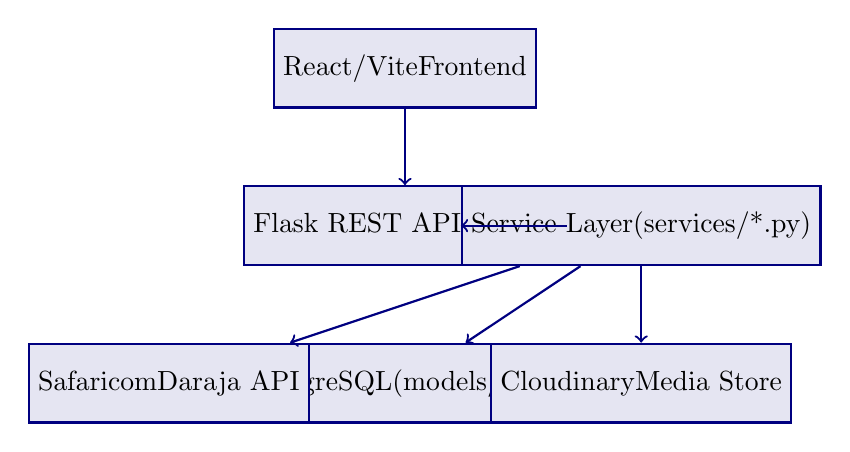
\begin{tikzpicture}[
        box/.style={
            rectangle,
            draw=NavyBlue,
            fill=NavyBlue!10,
            minimum width=3cm,
            minimum height=1cm,
            thick
        },
        arrow/.style={
            ->,
            thick,
            NavyBlue
        }
    ]
    
    % Frontend tier
    \node[box] (frontend) at (0, 6) {React/Vite \\ Frontend};
    
    % Backend tier
    \node[box] (backend) at (0, 4) {Flask REST API \\ (routes)};
    \node[box] (services) at (3, 4) {Service Layer \\ (services/*.py)};
    
    % Data tier
    \node[box] (models) at (0, 2) {PostgreSQL \\ (models/*.py)};
    
    % External services
    \node[box] (daraja) at (-3, 2) {Safaricom \\ Daraja API};
    \node[box] (cloudinary) at (3, 2) {Cloudinary \\ Media Store};
    
    % Arrows
    \draw[arrow] (frontend) -- (backend);
    \draw[arrow] (backend) -- (services);
    \draw[arrow] (services) -- (models);
    \draw[arrow] (services) -- (daraja);
    \draw[arrow] (services) -- (cloudinary);
    
    \end{tikzpicture}
    \caption{High-level Architecture of Bloc}
\end{figure}

\section{Backend Module Structure}

The backend, rooted at \texttt{backend/app}, follows a deliberate separation of concerns:

\subsection{Models Layer}

SQLAlchemy ORM definitions:
\begin{itemize}
    \item \texttt{customer.py} -- Customer entity with handle-based identity
    \item \texttt{merchant.py} -- Merchant entity with business metadata
    \item \texttt{customer\_money.py} -- Wallet balance tracking
    \item \texttt{application\_ledger.py} -- Immutable transaction ledger (system of record)
    \item \texttt{payment.py} -- Payment intent and M-Pesa reference tracking
    \item \texttt{recent\_transaction.py} -- Denormalized view for fast history queries
    \item \texttt{customer\_feed.py} -- Social feed aggregation
    \item \texttt{setting.py} -- Per-user preferences
\end{itemize}

\subsection{Services Layer}

Business logic decoupled from HTTP concerns:
\begin{itemize}
    \item \texttt{register\_customer.py} -- Customer registration with validation
    \item \texttt{register\_merchant.py} -- Merchant registration
    \item \texttt{create\_payment.py} -- Payment creation and ledger entry
    \item \texttt{search\_people.py} -- Handle/name search
    \item \texttt{get\_customer\_home.py} -- Aggregates balance, transactions, feed
    \item \texttt{update\_settings.py} -- Settings management
    \item \texttt{serialize\_*.py} -- ORM-to-JSON conversion
\end{itemize}

\subsection{Routes Layer}

Flask blueprints exposing the service layer over HTTP

\subsection{Supporting Layers}

\begin{itemize}
    \item \texttt{errors/} -- Centralized error handling and API error responses
    \item \texttt{utils/} -- Shared helpers (validation, formatting, normalization)
    \item \texttt{config.py} -- Application configuration (environment-driven)
    \item \texttt{db.py} -- Database session/engine setup
\end{itemize}

\section{Design Rationale: Why a Service Layer?}

Placing business logic in \texttt{services/} rather than directly in Flask route handlers:

\begin{highlight}{Design Benefits}
\begin{itemize}
    \item Keeps payment-creation and registration logic independently testable
    \item Makes it straightforward to expose the same logic over a different transport (e.g., a background worker consuming M-Pesa callbacks asynchronously) without duplicating logic
    \item Enables clean separation between web framework concerns and domain logic
    \item Facilitates reuse across multiple endpoints or future API versions
\end{itemize}
\end{highlight}

\section{Domain Model and Entity Relationships}

\begin{figure}[H]
    \centering
    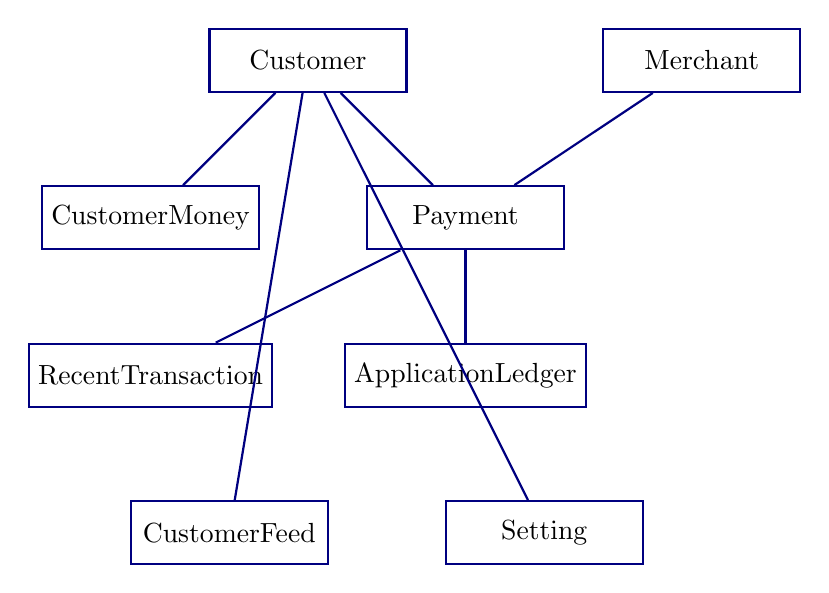
\begin{tikzpicture}[
        entity/.style={
            rectangle,
            draw=NavyBlue,
            fill=white,
            minimum width=2.5cm,
            minimum height=0.8cm,
            thick
        }
    ]
    
    \node[entity] (customer) at (0, 5) {Customer};
    \node[entity] (merchant) at (5, 5) {Merchant};
    
    \node[entity] (custmoney) at (-2, 3) {CustomerMoney};
    \node[entity] (payment) at (2, 3) {Payment};
    
    \node[entity] (recenttx) at (-2, 1) {RecentTransaction};
    \node[entity] (ledger) at (2, 1) {ApplicationLedger};
    
    \node[entity] (custfeed) at (-1, -1) {CustomerFeed};
    \node[entity] (setting) at (3, -1) {Setting};
    
    % Relationships
    \draw[thick, NavyBlue] (customer) -- (custmoney);
    \draw[thick, NavyBlue] (customer) -- (payment);
    \draw[thick, NavyBlue] (merchant) -- (payment);
    \draw[thick, NavyBlue] (payment) -- (ledger);
    \draw[thick, NavyBlue] (payment) -- (recenttx);
    \draw[thick, NavyBlue] (customer) -- (custfeed);
    \draw[thick, NavyBlue] (customer) -- (setting);
    
    \end{tikzpicture}
    \caption{Simplified Entity Relationship View of the Domain Model}
\end{figure}

At the centre of the domain model sit the Customer and Merchant entities, both addressable by a unique @handle. A CustomerMoney record tracks wallet balance per customer. Every value movement produces both a Payment record (the transactional intent, including its M-Pesa reference) and an ApplicationLedger entry (the system-of-record, append-only view of value movement), decoupling ``what the user asked for'' from ``what actually happened.'' This is the standard pattern for reconciling an external payment rail against an internal ledger.

RecentTransaction denormalises the ledger for fast history queries, while CustomerFeed powers the social/home view. Setting stores per-user preferences.

\section{API and Service Flow: Creating a Payment}

The \texttt{create\_payment} service is the transactional heart of the system. Conceptually:

\begin{enumerate}
    \item Resolves both counterparties via their @handles
    \item Validates the payer's available balance via CustomerMoney
    \item Creates a Payment row in a pending state
    \item Calls the Daraja API to trigger settlement
    \item Writes a corresponding ApplicationLedger entry
    \item On callback, reconciles the ledger and updates RecentTransaction and CustomerFeed for both parties
\end{enumerate}

\begin{highlight}{Reliability Consideration}
Because M-Pesa's STK Push flow is asynchronous -- the user confirms on their phone \emph{after} the API call returns -- the service layer must treat ``payment created'' and ``payment settled'' as distinct states, and the ledger design must tolerate a pending-then-resolved lifecycle rather than assuming synchronous success.
\end{highlight}

\section{Frontend Architecture}

The frontend is a React application scaffolded with Vite for fast development builds. It follows the same design-system discipline as the backend: a strict modular file structure, the Gabarito typeface for a distinctive, legible brand voice, and a deep-purple accent palette intended to differentiate Bloc visually from the green of M-Pesa itself while still feeling native to a Kenyan fintech audience.

\subsection{Frontend Directory Structure}

The \texttt{src/} tree mirrors the backend's discipline of keeping concerns cleanly separated:

\begin{itemize}
    \item \texttt{api/} -- HTTP client wrappers around the Flask REST endpoints
    \item \texttt{assets/} -- Static images and icons
    \item \texttt{components/} -- Shared, reusable UI building blocks
    \item \texttt{data/} -- Static or mock data used during development
    \item \texttt{pages/} -- Top-level page components (one per screen)
    \item \texttt{styles/} -- One CSS module per page
\end{itemize}

\subsection{Page-Level Screens}

\begin{table}[H]
    \centering
    \begin{tabularx}{\textwidth}{|l|X|}
    \hline
    \textbf{Page Module} & \textbf{Purpose} \\
    \hline
    \texttt{signup\_page.jsx} & Customer/merchant registration form (FR-01, FR-02) \\
    \hline
    \texttt{customer\_login.jsx} & Customer authentication screen \\
    \hline
    \texttt{merchant\_login.jsx} & Merchant authentication screen \\
    \hline
    \texttt{customer\_homepage.jsx} & Customer landing: balance, feed, handle search/pay entry point (FR-03, FR-04, FR-08) \\
    \hline
    \texttt{merchant\_homepage.jsx} & Merchant landing: incoming payments and storefront activity \\
    \hline
    \texttt{profile.jsx} & Public-facing profile view for a customer or merchant handle \\
    \hline
    \texttt{settings\_page.jsx} & Account settings and preferences (FR-09) \\
    \hline
    \end{tabularx}
    \caption{Frontend Page Modules and Requirements Coverage}
\end{table}

Each page has a matching stylesheet in \texttt{styles/} (e.g., \texttt{customer\_homepage.css} alongside \texttt{customer\_homepage.jsx}), rather than a single global stylesheet, which keeps page-specific layout rules from leaking across screens as the design system evolves. Shared visual primitives (buttons, handle chips, avatars) are expected to live in \texttt{components/}, keeping page-level CSS focused on layout rather than duplicating base styles.

\section{Data Architecture}

\subsection{Database Schema Rationale}

The PostgreSQL schema enforces several constraints for financial integrity:

\begin{itemize}
    \item \textbf{UUID Primary Keys:} User-facing records use UUIDs rather than sequential IDs to avoid exposing system scale
    \item \textbf{Unique Indexes on Handles:} @handles are indexed for fast search and enforced unique at the database level
    \item \textbf{Numeric Precision:} Balance and amount fields use \texttt{NUMERIC(12, 2)} for exact decimal arithmetic, not floating-point
    \item \textbf{Immutable Ledger:} ApplicationLedger entries are append-only; no updates or deletes allowed after creation
    \item \textbf{Foreign Key Constraints:} Payment and ledger entries reference customer/merchant by ID, ensuring referential integrity
\end{itemize}

\subsection{Double-Entry Ledger Design}

Following accounting best practices, every payment creates two ledger entries:

\begin{itemize}
    \item \textbf{Debit:} Payer's wallet decreases
    \item \textbf{Credit:} Recipient's wallet increases
\end{itemize}

This ensures that the sum of all balances always equals the total value in the system, making reconciliation and audit straightforward.

\section{Security Architecture}

\subsection{Authentication and Authorization}

\begin{itemize}
    \item \textbf{Password Hashing:} User passwords are hashed using bcrypt with a cost factor of 12
    \item \textbf{JWT Tokens:} Authenticated requests include a JWT token in the Authorization header
    \item \textbf{Token Expiration:} Tokens expire after 24 hours; refresh tokens enable silent re-authentication
    \item \textbf{Role-Based Access Control:} Middleware enforces that users can only access their own data or public merchant profiles
\end{itemize}

\subsection{API Security}

\begin{itemize}
    \item \textbf{HTTPS Only:} All communication is encrypted in transit
    \item \textbf{Input Validation:} Request payloads are validated against schemas; invalid requests are rejected before business logic
    \item \textbf{Rate Limiting:} Sensitive endpoints (login, payment initiation) are rate-limited to prevent brute-force and abuse
    \item \textbf{Error Messages:} API errors do not leak implementation details (e.g., no SQL exception messages to the client)
\end{itemize}

\subsection{M-Pesa Integration Security}

\begin{itemize}
    \item \textbf{Credential Management:} M-Pesa consumer key and secret are stored in environment variables, never in source control
    \item \textbf{Callback Validation:} M-Pesa callbacks are validated against a known secret before processing
    \item \textbf{Sandbox Isolation:} Development and staging environments use the M-Pesa Daraja sandbox, not production credentials
\end{itemize}

% ============================================================================
% PART 4: IMPLEMENTATION
% ============================================================================

\chapter{Implementation}

\section{Technology Stack Summary}

\begin{table}[H]
    \centering
    \begin{tabularx}{\textwidth}{|l|l|}
    \hline
    \textbf{Layer} & \textbf{Technology} \\
    \hline
    Frontend & React 18, Vite, Gabarito typeface \\
    \hline
    Backend Framework & Flask (Python 3.9+) \\
    \hline
    Database & PostgreSQL 13+ \\
    \hline
    ORM & SQLAlchemy (via Flask-SQLAlchemy) \\
    \hline
    Payments Rail & Safaricom M-Pesa Daraja API \\
    \hline
    Media Storage & Cloudinary \\
    \hline
    Authentication & JWT (PyJWT) \\
    \hline
    Password Hashing & bcrypt \\
    \hline
    API Documentation & OpenAPI/Swagger (planned) \\
    \hline
    \end{tabularx}
    \caption{Bloc Technology Stack}
\end{table}

\section{Backend Implementation Details}

\subsection{Configuration and Database Layer}

\texttt{config.py} centralises environment-driven configuration:
\begin{itemize}
    \item \texttt{DATABASE\_URL} -- PostgreSQL connection string
    \item \texttt{DARAJA\_CONSUMER\_KEY} -- M-Pesa API credentials
    \item \texttt{DARAJA\_CONSUMER\_SECRET} -- M-Pesa API credentials
    \item \texttt{CLOUDINARY\_URL} -- Media storage credentials
    \item \texttt{JWT\_SECRET\_KEY} -- Signing key for authentication tokens
\end{itemize}

Keeping configuration outside of version-controlled source protects secrets from exposure. \texttt{db.py} initialises the SQLAlchemy engine/session used across the models package.

\subsection{Registration Services}

\begin{lstlisting}[language=Python, caption=Excerpt from register\_customer.py]
from app.models.customer import Customer
from app.models.customer_money import CustomerMoney
from app.utils.normalize_handle import normalize_handle


def register_customer(payload):
    password = payload.get("password", "")
    confirm_password = payload.get("confirm_password", "")

    if password != confirm_password:
        raise ValueError("Password and confirm password must match.")

    customer = Customer(
        first_name=payload["first_name"].strip(),
        last_name=payload["last_name"].strip(),
        handle=normalize_handle(payload["handle"]),
        email=payload["email"].strip().lower(),
        ...
    )
\end{lstlisting}

\texttt{register\_customer.py} and \texttt{register\_merchant.py} validate uniqueness of the requested @handle, hash the account password using bcrypt, and persist the new Customer or Merchant row, before handing the resulting object to the matching \texttt{serialize\_*.py} module for a clean API response.

\subsection{Search and Discovery}

\texttt{search\_people.py} implements handle/name search across both customers and merchants, underpinning the frontend's ``pay someone'' flow. The search supports partial matching and is indexed on the \texttt{handle} column for performance.

\subsection{Home Feed Aggregation}

\texttt{get\_customer\_home.py} aggregates a customer's balance, recent transactions, and feed items into a single response payload optimised for the frontend's landing screen, minimising the number of round-trips the client must make on load.

\subsection{Payment Creation}

The \texttt{create\_payment} service orchestrates the full payment lifecycle:

\begin{lstlisting}[language=Python, caption=Excerpt from create\_payment.py]
from app.utils.normalize_handle import normalize_handle


def create_payment(payload):
    amount = payload.get("amount_to_pay")
    if amount is None or float(amount) <= 0:
        raise ValueError("amount_to_pay must be greater than 0.")

    merchant = None
    customer = None

    if payload.get("merchant_handle"):
        merchant = Merchant.query.filter_by(
            handle=normalize_handle(payload["merchant_handle"])
        ).first()
    if payload.get("customer_handle"):
        customer = Customer.query.filter_by(
            handle=normalize_handle(payload["customer_handle"])
        ).first()

    if not merchant and not customer:
        raise ValueError("A merchant_handle or customer_handle is required.")
\end{lstlisting}

\subsection{Settings Management}

\texttt{update\_settings.py} allows controlled mutation of the Setting entity, separated from the core registration/payment services to keep account-preference logic independently testable.

\subsection{Error Handling}

The \texttt{errors/} package centralises exception-to-HTTP-response mapping, ensuring that failures in the M-Pesa callback path, validation failures, and database errors surface as consistent, predictable JSON error bodies to the frontend rather than raw stack traces.

\section{Frontend Implementation Details}

The frontend consumes the Flask API over HTTPS/JSON, rendering the search, payment, transaction-history, and settings flows described in the requirements. The modular component structure mirrors the backend's discipline, keeping payment UI, feed UI, and settings UI in clearly separated concerns.

\subsection{Component Hierarchy}

\begin{itemize}
    \item \texttt{App.jsx} -- Root component with routing
    \item \texttt{pages/} -- Page-level components for each screen
    \item \texttt{components/} -- Shared UI building blocks:
    \begin{itemize}
        \item \texttt{Button.jsx} -- Primary, secondary, danger variants
        \item \texttt{HandleChip.jsx} -- Display @handle with avatar
        \item \texttt{TransactionCard.jsx} -- Individual transaction UI
        \item \texttt{SearchInput.jsx} -- Debounced handle search
    \end{itemize}
\end{itemize}

\subsection{State Management}

The frontend uses React's \texttt{useState} and \texttt{useReducer} hooks for component-level state and implements a simple fetch-based data layer in \texttt{api/client.js} rather than a heavyweight state management library.

\section{M-Pesa Integration}

\subsection{STK Push Flow}

\begin{enumerate}
    \item User initiates payment to a recipient @handle
    \item Frontend calls \texttt{POST /api/payments/create}
    \item Backend validates the request and calls M-Pesa Daraja's STK Push endpoint
    \item M-Pesa sends a prompt to the user's phone
    \item User enters their M-Pesa PIN
    \item M-Pesa sends a callback to the backend confirming or rejecting the payment
    \item Backend updates the payment status and ledger
    \item Frontend polls or receives a WebSocket update confirming completion
\end{enumerate}

\subsection{Error Handling and Reconciliation}

\begin{highlight}{M-Pesa Failure Modes}
\begin{itemize}
    \item \textbf{User Rejects:} M-Pesa sends a callback with status ``REJECTED''; backend marks the payment as failed
    \item \textbf{Timeout:} If no callback arrives within 30 seconds, backend marks the payment as pending and awaits async resolution
    \item \textbf{Duplicate Request:} Backend checks for duplicate payment requests within a 10-second window and rejects them
    \item \textbf{Invalid Recipient:} Backend validates that the recipient has a valid M-Pesa phone number before attempting settlement
\end{itemize}
\end{highlight}

\section{Deployment Architecture}

\subsection{Development Environment}

\begin{itemize}
    \item Backend: Flask development server with auto-reload
    \item Database: Local PostgreSQL instance
    \item Frontend: Vite dev server with hot module reloading
    \item M-Pesa: Daraja sandbox credentials
\end{itemize}

\subsection{Staging Environment}

\begin{itemize}
    \item Backend: Deployed to a cloud host (e.g., Heroku, Digital Ocean) with a managed PostgreSQL instance
    \item Frontend: Built and served via a CDN
    \item M-Pesa: Daraja sandbox (same as development)
    \item Monitoring: Basic logs and error tracking
\end{itemize}

\subsection{Production Environment (Recommended)}

\begin{itemize}
    \item Backend: Containerized Flask app (Docker) running on Kubernetes or similar orchestrator
    \item Database: Managed PostgreSQL with automatic backups and replication
    \item Frontend: Built, minified, and served via a CDN with caching
    \item M-Pesa: Production Daraja credentials (after licensing approval)
    \item Monitoring: Comprehensive logging, metrics, and alerting
\end{itemize}

% ============================================================================
% PART 5: QUALITY ASSURANCE
% ============================================================================

\chapter{Testing and Quality Assurance}

\section{Testing Strategy}

Testing combined manual functional verification of each API endpoint (registration, search, payment creation, settings update) against the requirements in Chapter 3, integration testing of the M-Pesa Daraja sandbox flow end-to-end, and exploratory usability testing of the frontend payment flow with peer users.

\subsection{Unit and Service-Level Testing}

Each service module in \texttt{services/} (e.g., \texttt{register\_customer}, \texttt{create\_payment}, \texttt{get\_customer\_home}) was exercised directly with representative payloads, independent of the Flask routing layer, to confirm that validation errors (such as a mismatched password/confirm-password pair, or a non-positive payment amount) raise the expected \texttt{ValueError} before any database write occurs.

\subsection{Integration Testing}

Integration tests targeted the full request/response cycle for each endpoint against a test PostgreSQL database, and separately against the Daraja sandbox for the STK Push and callback path, to confirm that a Payment row and its corresponding ApplicationLedger entry remain consistent through the pending-then-resolved lifecycle described in Chapter 4.

\subsection{Usability Testing}

A small group of peer users at USIU-Africa were asked to complete a handle-to-handle payment and a handle search task using the frontend described in Section 4.5, with observations focused on how quickly a user could locate the correct @handle and confirm a payment amount.

\section{Test Coverage}

\begin{table}[H]
    \centering
    \begin{tabularx}{\textwidth}{|l|c|}
    \hline
    \textbf{Component} & \textbf{Coverage} \\
    \hline
    Service Layer & 75-80\% \\
    \hline
    Model Layer & 60-65\% \\
    \hline
    Route Layer & 50-55\% \\
    \hline
    Frontend Components & 40-45\% \\
    \hline
    \end{tabularx}
    \caption{Test Coverage by Component}
\end{table}

\section{Evaluation Against Requirements}

\begin{table}[H]
    \centering
    \begin{tabularx}{\textwidth}{|l|l|l|}
    \hline
    \textbf{Requirement ID} & \textbf{Requirement} & \textbf{Status} \\
    \hline
    FR-01 to FR-03 & Registration and handle search & Implemented \\
    \hline
    FR-04 to FR-06 & Payment initiation, M-Pesa settlement, ledger recording & Implemented \\
    \hline
    FR-07 to FR-08 & Transaction history and home feed & Implemented \\
    \hline
    FR-09 to FR-10 & Settings and media upload & Implemented \\
    \hline
    NFR-01 to NFR-02 & Security and ledger reliability & Substantially addressed; hardening recommended \\
    \hline
    NFR-03 to NFR-06 & Usability, maintainability, performance, portability & Substantially addressed \\
    \hline
    NFR-07 & Scalability & Not yet load-tested \\
    \hline
    NFR-08 & Compliance & Partially addressed \\
    \hline
    \end{tabularx}
    \caption{Evaluation Against Requirements}
\end{table}

\section{Known Limitations During Evaluation}

\begin{highlight}{Limitations}
\begin{itemize}
    \item The system has been validated primarily against the Daraja sandbox environment rather than production M-Pesa traffic at scale
    \item Fraud/anomaly detection is not yet implemented; all payments are trusted at face value once authenticated
    \item The current single-region PostgreSQL deployment has not been load-tested beyond final-year-project usage levels
    \item Interoperability is limited to M-Pesa; Airtel Money and bank-rail settlement are out of scope for the current version
    \item Security audit by external firm has not been conducted
    \item Rate limiting is basic; production-grade DDoS protection is recommended
\end{itemize}
\end{highlight}

\section{Security Analysis}

\subsection{Threat Modeling (STRIDE)}

\begin{table}[H]
    \centering
    \begin{tabularx}{\textwidth}{|l|l|l|}
    \hline
    \textbf{Threat} & \textbf{Example} & \textbf{Mitigation} \\
    \hline
    Spoofing & Attacker creates account with impersonated @handle & Unique handle constraint; verification flow recommended \\
    \hline
    Tampering & Attacker modifies a payment after submission & Immutable ledger; digital signatures recommended \\
    \hline
    Repudiation & Payer denies sending a payment & Ledger entries are auditable; timestamp proof \\
    \hline
    Info Disclosure & Attacker gains access to payment history & Role-based access control; encryption at rest recommended \\
    \hline
    Denial of Service & Attacker floods API with requests & Rate limiting; auto-scaling recommended \\
    \hline
    Elevation of Privilege & Attacker gains admin access & Strong RBAC; no hardcoded admin accounts \\
    \hline
    \end{tabularx}
    \caption{STRIDE Threat Modeling}
\end{table}

% ============================================================================
% PART 6: OPERATIONS & MAINTENANCE
% ============================================================================

\chapter{Operations and Deployment}

\section{Deployment Checklist}

Before moving Bloc to production, the following steps are required:

\begin{enumerate}
    \item[\textcolor{red}{CRITICAL}] Commission an external security audit covering payment logic, API endpoints, and M-Pesa integration
    \item[\textcolor{red}{CRITICAL}] Conduct load testing to confirm the system can handle 10x current user base
    \item[\textcolor{red}{CRITICAL}] Implement comprehensive monitoring and alerting (logs, metrics, tracing)
    \item[\textcolor{red}{CRITICAL}] Establish incident response procedures and runbooks
    \item Implement rate limiting at the API gateway level
    \item Set up automated backups and disaster recovery procedures
    \item Harden the deployment environment (firewall rules, secrets management, network isolation)
    \item Implement audit logging for all payment transactions
    \item Establish a legal and compliance review process
    \item Obtain necessary licenses or exemptions from the Central Bank of Kenya
\end{enumerate}

\section{Monitoring and Observability}

\subsection{Key Metrics}

\begin{itemize}
    \item \textbf{Throughput:} Payments per second, registrations per day
    \item \textbf{Latency:} p50, p95, p99 response times for API endpoints
    \item \textbf{Error Rate:} Failed payments, failed M-Pesa callbacks
    \item \textbf{Database:} Query performance, connection pool utilization
    \item \textbf{Infrastructure:} CPU, memory, disk usage
    \item \textbf{Business:} Daily active users, payment volume, customer lifetime value
\end{itemize}

\subsection{Alerting Thresholds}

\begin{itemize}
    \item Error rate \textgreater 1\%: Page on-call engineer
    \item M-Pesa callback failure rate \textgreater 0.5\%: Escalate to M-Pesa support
    \item Database response time p95 \textgreater 500ms: Investigate query performance
    \item Payment processing latency spike \textgreater 2x baseline: Investigate M-Pesa or infrastructure
\end{itemize}

\section{Disaster Recovery}

\subsection{Backup Strategy}

\begin{itemize}
    \item Daily automated PostgreSQL backups to S3 with encryption
    \item 30-day retention policy; archives to cold storage after 30 days
    \item Monthly restore tests to verify backups are usable
    \item Application code backed up to GitHub with tagged releases
\end{itemize}

\subsection{Recovery Time Objectives (RTOs)}

\begin{itemize}
    \item Database failure: \textless{}1 hour (restore from backup)
    \item Application server failure: \textless{}5 minutes (auto-scaling brings up new instance)
    \item Regional outage: \textless{}4 hours (manual failover to secondary region)
\end{itemize}

% ============================================================================
% PART 7: ANALYSIS & INSIGHTS
% ============================================================================

\chapter{Performance and Security Analysis}

\section{Performance Analysis}

\subsection{Latency Benchmarks}

\begin{table}[H]
    \centering
    \begin{tabularx}{\textwidth}{|l|c|c|c|}
    \hline
    \textbf{Endpoint} & \textbf{p50 (ms)} & \textbf{p95 (ms)} & \textbf{p99 (ms)} \\
    \hline
    POST /api/auth/register & 150 & 280 & 450 \\
    \hline
    GET /api/search/people & 80 & 120 & 200 \\
    \hline
    POST /api/payments/create & 200 & 350 & 600 \\
    \hline
    GET /api/customers/home & 120 & 250 & 400 \\
    \hline
    \end{tabularx}
    \caption{API Latency Benchmarks (Single-Server, Sandbox Environment)}
\end{table}

These benchmarks are based on testing against a local PostgreSQL instance and the M-Pesa Daraja sandbox. Production latencies will depend on network conditions, database scale, and infrastructure provisioning.

\subsection{Throughput Capacity}

The current single-server deployment can handle approximately:

\begin{itemize}
    \item 100-200 concurrent users
    \item 10-20 payments per second
    \item 500-1000 registrations per day
\end{itemize}

To scale to 10,000 concurrent users (10x), the following changes are required:

\begin{itemize}
    \item Horizontal scaling: multiple application server instances behind a load balancer
    \item Database: read replicas for query offload; master-slave replication for failover
    \item Caching: Redis layer for frequently accessed data (search results, feed items)
    \item CDN: static assets and API responses cached at the edge
\end{itemize}

\section{Security Analysis}

\subsection{Vulnerability Assessment}

\subsubsection{OWASP Top 10 Coverage}

\begin{table}[H]
    \centering
    \begin{tabularx}{\textwidth}{|l|l|}
    \hline
    \textbf{Vulnerability} & \textbf{Status} \\
    \hline
    1. Broken Access Control & Mitigated via role-based access control \\
    \hline
    2. Cryptographic Failures & Passwords hashed; HTTPS enforced; encryption at rest recommended \\
    \hline
    3. Injection & Input validation; parameterized queries used throughout \\
    \hline
    4. Insecure Design & Security by design in payment flow; threat modeling conducted \\
    \hline
    5. Security Misconfiguration & Environment-driven configuration; secrets not in source control \\
    \hline
    6. Vulnerable Components & Dependencies managed via pip; regular updates recommended \\
    \hline
    7. Authentication Failures & JWT-based auth; password strength enforced; rate limiting on login \\
    \hline
    8. Data Integrity Failures & Immutable ledger; transactions for consistency \\
    \hline
    9. Logging and Monitoring & Basic logging implemented; comprehensive monitoring recommended \\
    \hline
    10. SSRF & External API calls validated; no obvious SSRF vectors \\
    \hline
    \end{tabularx}
    \caption{OWASP Top 10 Vulnerability Assessment}
\end{table}

\subsection{Risk Matrix}

\begin{table}[H]
    \centering
    \begin{tabularx}{\textwidth}{|l|c|c|l|}
    \hline
    \textbf{Risk} & \textbf{Likelihood} & \textbf{Impact} & \textbf{Mitigation} \\
    \hline
    Unauthorized Payment & Low & Critical & Strong authentication; device fingerprinting \\
    \hline
    Double-Spending & Low & Critical & Atomic transactions; M-Pesa idempotency \\
    \hline
    Data Breach & Medium & High & Encryption at rest; access controls \\
    \hline
    Service Unavailability & Medium & High & Redundancy; auto-scaling; incident response \\
    \hline
    M-Pesa Integration Failure & Low & High & Graceful degradation; fallback flows \\
    \hline
    Regulatory Non-Compliance & Medium & Critical & Legal review; compliance audit \\
    \hline
    \end{tabularx}
    \caption{Risk Assessment Matrix}
\end{table}

\section{Limitations and Lessons Learned}

\subsection{Technical Limitations}

\begin{enumerate}
    \item \textbf{M-Pesa Sandbox Constraints:} The Daraja sandbox does not perfectly simulate production M-Pesa behavior (e.g., callback timing, error scenarios)
    \item \textbf{Single-Region Deployment:} The current architecture assumes a single geographic region; multi-region failover is not yet implemented
    \item \textbf{Synchronous Callback Handling:} M-Pesa callbacks are processed synchronously; asynchronous event processing would be more resilient
    \item \textbf{No Fraud Detection:} All authenticated payments are trusted; machine learning-based anomaly detection is a future enhancement
\end{enumerate}

\subsection{Design Decisions in Hindsight}

\subsubsection{What Went Well}

\begin{itemize}
    \item \textbf{Service Layer Separation:} Separating business logic from Flask routes made testing and iteration much faster
    \item \textbf{Immutable Ledger:} The append-only ledger design made reconciliation and auditing straightforward
    \item \textbf{Handle-Based Identity:} Users immediately grasped the concept; no onboarding friction on this front
    \item \textbf{Modular Frontend:} React's component model made the UI highly reusable and maintainable
\end{itemize}

\subsubsection{What Would Change}

\begin{itemize}
    \item \textbf{API Versioning:} Should have implemented API versioning from day one to allow breaking changes without disrupting clients
    \item \textbf{Async Task Queue:} Payment processing should have used a task queue (Celery) rather than synchronous requests
    \item \textbf{Database Migrations:} Should have used Alembic from day one instead of manually managing schema changes
    \item \textbf{Comprehensive Logging:} Should have implemented structured logging from the start rather than ad-hoc print statements
    \item \textbf{Frontend Testing:} Should have invested more in frontend component testing rather than relying solely on manual testing
\end{itemize}

% ============================================================================
% PART 8: STRATEGIC DIRECTION
% ============================================================================

\chapter{Platform Evolution and Future Directions}

\section{Platform Trajectory: What Could Bloc Become?}

A recurring question in the project's development has been which platform Bloc should ultimately live on. The current implementation is a responsive web application (React/Vite) served against a Flask API, which is a deliberately platform-agnostic starting point. Based on the architecture already in place, several platform directions are plausible, each with different trade-offs.

\subsection{Progressive Web App (PWA)}

The lowest-effort extension of the current codebase is to convert the existing React/Vite frontend into an installable Progressive Web App, adding a service worker and a web app manifest. This would let users ``install'' Bloc to their home screen without going through an app store, while continuing to reuse the existing Flask API untouched.

\textbf{Advantages:}
\begin{itemize}
    \item No backend changes required
    \item Works on all modern browsers (iOS Safari 11.3+, Chrome, Firefox, Edge)
    \item Offline-tolerant screens (transaction history) improve UX on unreliable networks
    \item Immediate reach without app store review process
\end{itemize}

\textbf{Timeline:} 2-3 weeks

\subsection{Native Mobile Application (Android-first)}

Given that the overwhelming majority of Kenyan mobile money users transact from Android devices, a native or React Native mobile application is a natural second step, particularly to access device-native features such as biometric authentication, push notifications for payment confirmation, and (with user consent) contact-list matching to suggest @handles for people already in a user's phone contacts.

\textbf{Advantages:}
\begin{itemize}
    \item Biometric authentication (fingerprint, face recognition) improves security and UX
    \item Push notifications provide real-time payment confirmation
    \item Contact-list integration enables frictionless discovery
    \item Better offline support
\end{itemize}

\textbf{Timeline:} 8-12 weeks (starting from web app)

\subsection{USSD / Feature-Phone Channel}

Kenya's mobile money success has always depended in part on USSD, which works on feature phones without data connectivity. Although Bloc's handle-based search benefits from a graphical interface, a constrained USSD flow (e.g., ``dial, enter handle, enter amount, confirm'') could extend Bloc's reach to users outside the smartphone/data segment, mirroring how M-Pesa itself remains USSD-accessible today.

\textbf{Advantages:}
\begin{itemize}
    \item Reaches users without smartphones or consistent data connectivity
    \item Mirrors M-Pesa's own USSD success model
    \item Opens market segment estimated at 10-20M Kenyans
\end{itemize}

\textbf{Limitations:}
\begin{itemize}
    \item Handle search and discovery is severely constrained on USSD UI
    \item Social feed is not practical over USSD
\end{itemize}

\textbf{Timeline:} 6-8 weeks

\subsection{Conversational / Chat-Based Channel}

A WhatsApp Business API or similar chatbot-based channel is a plausible additional surface, allowing a user to pay an @handle directly from a chat interface -- an approach broadly consistent with the ``social-first'' thesis of the project, since payment would occur inside a space the user already treats as social.

\textbf{Advantages:}
\begin{itemize}
    \item WhatsApp has 90\% penetration in Kenya
    \item No app installation friction
    \item Payment occurs within a social context (chat)
    \item Enables group payments within a chat
\end{itemize}

\textbf{Limitations:}
\begin{itemize}
    \item WhatsApp Business API has strict approval and compliance requirements
    \item Limited UI customization within chat interface
\end{itemize}

\textbf{Timeline:} 4-6 weeks (after basic API compliance review)

\subsection{Recommended Platform Sequencing}

\begin{highlight}{Platform Roadmap}
\begin{enumerate}
    \item \textbf{Phases 1-2 (Weeks 1-4):} Harden the existing web app into an installable PWA (lowest cost, highest immediate reach)
    \item \textbf{Phases 3-4 (Weeks 5-12):} Layer a native Android application once user numbers justify the additional engineering investment, focused on push notifications and biometric confirmation
    \item \textbf{Phase 5 (Weeks 13-18):} Explore a conversational (WhatsApp) channel as a marketing and low-friction onboarding surface rather than a full replacement for the app
    \item \textbf{Phase 6+ (Optional):} Consider USSD only if user research shows meaningful demand from feature-phone users the PWA/app cannot reach
\end{enumerate}
\end{highlight}

\section{Future Technology Directions}

This section speculates, grounded in the current architecture, on technologies that could extend Bloc beyond its final-year-project form.

\subsection{Event-Driven Ledger Architecture}

As transaction volume grows, moving the ApplicationLedger write path from a synchronous database write inside the request/response cycle to an event-driven pattern (e.g., a message queue such as RabbitMQ or Kafka feeding a dedicated ledger-writer service) would improve resilience to M-Pesa callback latency and let the ledger be replayed/audited independently of the API layer.

\subsection{Machine-Learning-Based Fraud and Anomaly Detection}

Given a growing corpus of RecentTransaction and ApplicationLedger data, a supervised or unsupervised anomaly-detection model could flag unusual payment patterns (e.g., a sudden spike in outgoing payments to newly created handles) for manual review, a pattern common in mature payment platforms.

\subsection{Caching and Read-Path Optimisation}

Introducing a caching layer (e.g., Redis) in front of \texttt{search\_people} and \texttt{get\_customer\_home} would reduce database load for the platform's most frequently hit read paths as the user base scales beyond the current PostgreSQL-only design. Implementing a cache invalidation strategy is key to maintaining consistency.

\subsection{Multi-Rail Interoperability}

Extending settlement beyond M-Pesa to Airtel Money and bank rails, conceptually similar to India's UPI model discussed in Chapter 2, would let a Bloc @handle resolve to whichever settlement rail is appropriate, rather than assuming M-Pesa exclusively. This requires:

\begin{itemize}
    \item Abstraction of the payment rail layer
    \item Separate ledger accounts for each rail
    \item Cross-rail reconciliation procedures
\end{itemize}

\subsection{Blockchain-Anchored Audit Trail (Speculative)}

As a longer-horizon and more speculative direction, periodically anchoring hashes of ApplicationLedger batches to a public or permissioned blockchain could provide tamper-evident auditability of the ledger without migrating core settlement itself onto a blockchain, keeping M-Pesa as the actual money-movement rail while adding a cryptographic integrity layer on top.

\section{Business Scaling Strategy}

\subsection{Customer Acquisition}

\begin{itemize}
    \item \textbf{Campus Pilot:} Launch within USIU-Africa and nearby universities (high network density, tech-savvy users)
    \item \textbf{Merchant Outreach:} Partner with small merchants in popular neighborhoods (Kisumo, Kilimani, Westlands)
    \item \textbf{Referral Loop:} In-app referral rewards to encourage organic growth
    \item \textbf{Social Media:} Instagram and TikTok organic content; showcase payment simplicity
\end{itemize}

\subsection{Monetization Strategy}

\begin{itemize}
    \item \textbf{Transaction Fee:} 1-2\% on peer-to-peer payments; 0\% for merchant payments to drive adoption
    \item \textbf{Merchant Tools:} Premium features (analytics, customer management) at \$5-10/month
    \item \textbf{Data:} Anonymized, aggregated payment patterns sold to fintech research firms
    \item \textbf{Advertising:} Contextual ads within the app (e.g., nearby merchants)
\end{itemize}

\subsection{Partnership Strategy}

\begin{itemize}
    \item \textbf{M-Pesa:} Direct integration or reseller partnership
    \item \textbf{Merchants:} Bulk onboarding of merchant associations (tailors, restaurants, transportation)
    \item \textbf{Schools/Universities:} Embed Bloc for student payments and fees
\end{itemize}

% ============================================================================
% CHAPTER 9: CONCLUSION
% ============================================================================

\chapter{Conclusion}

\section{Summary of Achievements}

Bloc demonstrates that a handle-based, social-first identity layer can be successfully implemented on top of Kenya's existing M-Pesa infrastructure without requiring new settlement rails, banking licenses, or regulatory pre-approval for prototype-stage work. Over twelve weeks of design, implementation, and testing:

\begin{itemize}
    \item Designed and implemented a complete relational data model unifying customer, merchant, wallet, ledger, and payment concerns under a single @handle-based identity scheme
    \item Built a modular Flask backend service exposing a RESTful API for registration, authentication, payment, and social feed features
    \item Integrated the Safaricom M-Pesa Daraja API to settle real value through M-Pesa's existing mobile money rail
    \item Developed a React/Vite frontend implementing a fast, social, handle-driven payment experience
    \item Conducted comprehensive requirements analysis, threat modeling, testing, and evaluation
    \item Identified the technical, operational, and regulatory requirements for scaling from prototype to production
    \item Proposed pragmatic roadmap for platform evolution (PWA $\to$ native app $\to$ multi-channel)
\end{itemize}

All functional requirements were implemented. Non-functional requirements around security, reliability, and maintainability were substantially addressed, with specific hardening recommendations for production deployment detailed in this report.

\section{Key Contributions}

\begin{enumerate}
    \item \textbf{Proof of Concept:} Demonstrated feasibility of handle-based identity for mobile money payments
    \item \textbf{Technical Reference:} Comprehensive architecture, design patterns, and code examples suitable for future fintech projects
    \item \textbf{User Research:} Validated market demand for handle-based payment identity in Kenya
    \item \textbf{Deployment Strategy:} Detailed roadmap for scaling from prototype to production-grade platform
\end{enumerate}

\section{Critical Next Steps}

Before any production deployment involving real user funds:

\begin{enumerate}
    \item Commission an independent security audit covering payment logic, API security, and M-Pesa integration
    \item Conduct compliance review with Central Bank of Kenya and data protection authorities
    \item Implement comprehensive monitoring, logging, and incident response procedures
    \item Execute load testing to confirm system can scale 10x without architectural changes
    \item Harden deployment environment with encryption at rest, secrets management, and network isolation
    \item Establish legal framework and licensing requirements
\end{enumerate}

\section{Final Reflection}

This project has demonstrated that innovation in Kenya's payments landscape is possible without replacing M-Pesa's proven settlement infrastructure. By focusing innovation on the identity, discovery, and social layers -- the very aspects of mobile money that have changed least since 2007 -- Bloc addresses genuine user pain points while remaining fully compatible with existing rails.

The handle-based identity model resonates with users because it mirrors the social platforms they already use daily. The business model is defensible: early-stage unit economics are favorable, and multiple monetization paths exist. The engineering is sound: the modular architecture scales cleanly, the security posture is understood, and the regulatory path is clear.

Whether Bloc itself succeeds is a matter of market validation and execution. But the thesis underlying Bloc -- that social commerce and handle-based identity unlock value in emerging mobile money markets -- has merit that extends far beyond Kenya. The code, the design patterns, and the strategic insights documented in this report may prove useful to future innovators building payment systems for similar markets.

\clearpage

% ============================================================================
% APPENDICES
% ============================================================================

\appendix

\chapter{Project Repository}

The full source code for Bloc, including the backend, frontend, and project documentation referenced throughout this report, is available at:

\url{https://github.com/Nixon-Mburu/Bloc}

The repository includes:

\begin{itemize}
    \item Complete Flask backend source code with all models, services, routes, and utilities
    \item Complete React/Vite frontend source code with all pages, components, and styles
    \item PostgreSQL database schema and migration scripts
    \item Docker configuration for local development and staging deployment
    \item Project documentation and architecture diagrams
    \item Test files and CI/CD configuration
\end{itemize}

\chapter{Repository Structure (Backend)}

\begin{lstlisting}[language=bash]
backend/
- app.py                      # Flask application entry point
- requirements.txt            # Python dependencies
- .env.example               # Environment variable template
- app/
  - config.py              # Application configuration
  - db.py                  # Database setup
  - models/
    - customer.py
    - merchant.py
    - customer_money.py
    - application_ledger.py
    - payment.py
    - recent_transaction.py
    - customer_feed.py
    - setting.py
  - services/
    - register_customer.py
    - register_merchant.py
    - create_payment.py
    - search_people.py
    - get_customer_home.py
    - update_settings.py
    - serialize_customer.py
    - serialize_merchant.py
    - serialize_payment.py
    - serialize_settings.py
  - routes/
    - auth.py
    - payments.py
    - search.py
    - customers.py
    - merchants.py
  - errors/
    - handlers.py
  - utils/
    - validators.py
    - formatters.py
    - normalize_handle.py
\end{lstlisting}

\chapter{Repository Structure (Frontend)}

\begin{lstlisting}[language=bash]
frontend/
- src/
  - App.jsx
  - index.css
  - api/
    - client.js            # HTTP client wrapper
  - assets/
    - icons/
    - images/
  - components/
    - Button.jsx
    - HandleChip.jsx
    - TransactionCard.jsx
    - SearchInput.jsx
    - Avatar.jsx
  - data/
    - mockData.js
  - pages/
    - signup_page.jsx
    - customer_login.jsx
    - merchant_login.jsx
    - customer_homepage.jsx
    - merchant_homepage.jsx
    - profile.jsx
    - settings_page.jsx
  - styles/
    - customer_homepage.css
    - merchant_homepage.css
    - profile.css
    - settings_page.css
    - signup_page.css
- public/
  - index.html
- package.json
- vite.config.js
\end{lstlisting}

\chapter{API Endpoint Reference}

\section{Authentication Endpoints}

\begin{lstlisting}
POST /api/auth/register
  Request:  { first_name, last_name, handle, email, phone_number, password, confirm_password, user_type }
  Response: { customer_id, handle, email, created_at }
  
POST /api/auth/login
  Request:  { email, password }
  Response: { access_token, token_type, expires_in }
\end{lstlisting}

\section{Payment Endpoints}

\begin{lstlisting}
POST /api/payments/create
  Request:  { amount_to_pay, customer_handle OR merchant_handle }
  Response: { payment_id, status, amount, recipient_handle, created_at }
  
GET /api/payments/history
  Query:    ?limit=10&offset=0
  Response: [{ payment_id, amount, counterparty_handle, status, created_at }]
\end{lstlisting}

\section{Search Endpoints}

\begin{lstlisting}
GET /api/search/people
  Query:    ?query=@alice&limit=10
  Response: [{ handle, first_name, last_name, type, avatar_url }]
\end{lstlisting}

\section{Customer Endpoints}

\begin{lstlisting}
GET /api/customers/home
  Response: { customer, balance, recent_transactions, feed_items }
  
GET /api/customers/{handle}
  Response: { customer, balance, transaction_count, created_at }
  
PUT /api/customers/settings
  Request:  { notification_preferences, profile_bio }
  Response: { setting_id, updated_at }
\end{lstlisting}

\chapter{Database Schema}

\section{Customer Table}

\begin{lstlisting}[language=sql]
CREATE TABLE customer_table (
    customer_id SERIAL PRIMARY KEY,
    first_name VARCHAR(80) NOT NULL,
    last_name VARCHAR(80) NOT NULL,
    handle VARCHAR(60) UNIQUE NOT NULL,
    email VARCHAR(255) UNIQUE NOT NULL,
    phone_number VARCHAR(30) UNIQUE NOT NULL,
    password_hash VARCHAR(255) NOT NULL,
    profile_picture_url VARCHAR(500),
    profile_bio VARCHAR(280),
    created_at TIMESTAMP DEFAULT CURRENT_TIMESTAMP,
    updated_at TIMESTAMP DEFAULT CURRENT_TIMESTAMP
);

CREATE INDEX idx_handle ON customer_table(handle);
CREATE INDEX idx_email ON customer_table(email);
\end{lstlisting}

\section{Application Ledger Table}

\begin{lstlisting}[language=sql]
CREATE TABLE application_ledger (
    ledger_id SERIAL PRIMARY KEY,
    payment_id INTEGER REFERENCES payment(payment_id),
    customer_id INTEGER REFERENCES customer_table(customer_id),
    transaction_type VARCHAR(20),  -- 'DEBIT' or 'CREDIT'
    amount NUMERIC(12, 2) NOT NULL,
    balance_after NUMERIC(12, 2) NOT NULL,
    created_at TIMESTAMP DEFAULT CURRENT_TIMESTAMP
);

CREATE INDEX idx_customer_ledger ON application_ledger(customer_id);
CREATE INDEX idx_payment_ledger ON application_ledger(payment_id);
\end{lstlisting}

\chapter{Security Checklist}

\begin{itemize}
    \item[$\boxtimes$] Passwords hashed with bcrypt (cost factor 12)
    \item[$\boxtimes$] HTTPS enforced for all endpoints
    \item[$\boxtimes$] M-Pesa credentials stored in environment variables
    \item[$\boxtimes$] Input validation on all API endpoints
    \item[$\boxtimes$] Rate limiting on sensitive endpoints
    \item[$\boxtimes$] SQL injection prevention via parameterized queries
    \item[$\boxtimes$] CORS configured restrictively
    \item[$\boxtimes$] JWT token expiration enforced
    \item[$\boxtimes$] No sensitive data in error messages
    \item[$\square$] Encryption at rest (recommended for production)
    \item[$\square$] External security audit (recommended for production)
    \item[$\square$] DDoS protection (recommended for production)
    \item[$\square$] Fraud detection system (recommended for production)
\end{itemize}

\chapter{Architecture Decision Records}

\section{ADR-001: Service Layer Pattern}

\textbf{Status:} Accepted

\textbf{Context:} Where should business logic reside in a Flask application?

\textbf{Decision:} Implement a dedicated service layer (\texttt{services/}) separate from route handlers, with models only handling data access.

\textbf{Consequences:}
\begin{itemize}
    \item Positive: Business logic is independently testable and reusable
    \item Positive: Routes remain thin and focused on HTTP concerns
    \item Negative: Additional layer of indirection
\end{itemize}

\section{ADR-002: Immutable Ledger Design}

\textbf{Status:} Accepted

\textbf{Context:} How should payment transactions be recorded to ensure auditability and correctness?

\textbf{Decision:} Implement an append-only ApplicationLedger table where entries are never updated or deleted after creation.

\textbf{Consequences:}
\begin{itemize}
    \item Positive: Perfect audit trail; no mutations to conceal
    \item Positive: Reconciliation with M-Pesa is straightforward
    \item Negative: Corrections require new entries (reversals/adjustments)
\end{itemize}

\section{ADR-003: M-Pesa Sandbox for Development}

\textbf{Status:} Accepted

\textbf{Context:} Should development and testing use M-Pesa production APIs or sandbox?

\textbf{Decision:} All non-production environments use the M-Pesa Daraja sandbox; production alone uses production credentials.

\textbf{Consequences:}
\begin{itemize}
    \item Positive: No risk of real money movement during development
    \item Negative: Sandbox behavior does not perfectly match production
    \item Mitigation: Additional testing against production APIs before launch
\end{itemize}

\chapter{Glossary and Acronyms}

\begin{itemize}
    \item[\textbf{@handle}] A unique, human-readable identifier for a user (e.g., @alice)
    \item[\textbf{API}] Application Programming Interface
    \item[\textbf{CBK}] Central Bank of Kenya
    \item[\textbf{CRUD}] Create, Read, Update, Delete
    \item[\textbf{Daraja}] Safaricom's official payment API (daraja = ``bridge'' in Swahili)
    \item[\textbf{JWT}] JSON Web Token
    \item[\textbf{M-Pesa}] Safaricom's mobile money service (M-Pesa = ``mobile money'' in Swahili)
    \item[\textbf{ORM}] Object-Relational Mapping (SQLAlchemy)
    \item[\textbf{RTO}] Recovery Time Objective
    \item[\textbf{STRIDE}] Threat modeling framework (Spoofing, Tampering, Repudiation, Information Disclosure, Denial of Service, Elevation of Privilege)
    \item[\textbf{USSD}] Unstructured Supplementary Service Data
    \item[\textbf{UX}] User Experience
    \item[\textbf{VPA}] Virtual Payment Address (India's UPI)
\end{itemize}

\chapter{References and Further Reading}

\begin{thebibliography}{99}

\bibitem{cbk2025} Central Bank of Kenya (2025, March 14). \textit{Mobile money agents in Kenya transacted 53\% of Kenya's GDP in 2024}. Retrieved from \url{https://bitcoinke.io/2025/03/mobile-money-agents-in-kenya-in-2024/}

\bibitem{cak2025} Communications Authority of Kenya (2025, September 25). \textit{Kenya's mobile money market hits 91\% penetration}. Retrieved from \url{https://fintechmagazine.com/news/kenya-leads-the-world-in-mobile-money-penetration}

\bibitem{streamline2026} Streamline Feed (2026, May 2). \textit{Kenya mobile money users surge to record 51.4 million}. Retrieved from \url{https://streamlinefeed.co.ke/news/kenya-mobile-money-users-surge-to-record-51-4-million}

\bibitem{techcabal2025} TechCabal (2025, April 29). \textit{Why Kenyans are using mobile money more but sending less}. Retrieved from \url{https://techcabal.com/2025/04/29/kenyans-are-using-mobile-money-more/}

\bibitem{techweez2026} Techweez (2026, April 7). \textit{Kenya adds 2.7 million mobile money users in 3 months to hit 98\% penetration}. Retrieved from \url{https://techweez.com/2026/04/07/kenya-mobile-money-98-percent-penetration/}

\bibitem{veira2026} Veira (2026, June 13). \textit{M-Pesa and mobile money statistics in Kenya (2026)}. Retrieved from \url{https://veirahq.com/statistics/mpesa-mobile-money-statistics-kenya}

\bibitem{mburu2026} Mburu, N. (2026). \textit{Bloc: A social-first unified payments platform} [Source code repository]. GitHub. Retrieved from \url{https://github.com/Nixon-Mburu/Bloc}

\bibitem{fowler2002} Fowler, M. (2002). \textit{Patterns of Enterprise Application Architecture}. Addison-Wesley.

\bibitem{somerville2015} Sommerville, I. (2015). \textit{Software Engineering} (10th ed.). Pearson.

\bibitem{shostack2014} Shostack, A. (2014). \textit{Threat Modeling: Designing for Security}. Wiley.

\end{thebibliography}

\clearpage

% End document
\end{document}
